\documentclass[UTF8]{ctexart}
\usepackage{graphicx}
\usepackage{amsmath}
\usepackage{bibentry,natbib}
\usepackage{fancyhdr}

\title{The theory in Word2Vec}
\author{BrightHush}
\date{\today}

\begin{document}
\maketitle
\tableofcontents

\pagestyle{fancy}
\cfoot{\thepage}

\newcommand{\figref}[1]{\figurename~\ref{#1}}

\section{Introduction}
Word2Vec中实现了两个模型,分别是CBOW(Continuous Bag of Words)模型和Skip-gram模型。
CBOW模型,在训练过程中是指给出了当前词的上下文,预测出现当前词的概率,其模型架构如图\ref{Fig:CBOW}。
而Sikp-gram模型,则是在给定当前词的情况下,计算上下文出现的概率,该模型可参见\ref{Fig:skipgram}。
\begin{figure}[h!]
    \centering     
    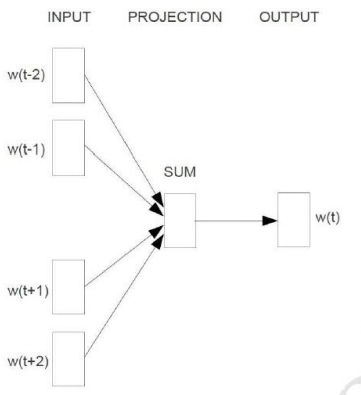
\includegraphics[width=0.5\textwidth]{cbow}   
    \caption{\label{Fig:CBOW}CBOW Architecture} 
\end{figure}

\begin{figure}[h!]
    \centering     
    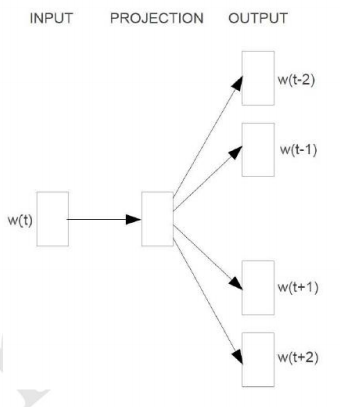
\includegraphics[width=0.5\textwidth]{skipgram}   
    \caption{\label{Fig:skipgram}Skip-gram Architecture} 
\end{figure}

\par
在word2vec中,分别基于 Hierarchical Softmax 和 Negative Sampling 的方法进行建模,下面的note
会详细讨论CBOW和Skip-gram在这两个方法下的细节。
\par
根据语言模型的定义,通常是给定上下文求出现下一个词的概率,基于这样的思路,在神经网络概率语言模型中,
我们也是需要建立这样的条件概率模型。因此COBW和Sikp-gram的log似然可以分别表示为(\ref{cobw-likelihood})
和(\ref{skipgram-likelihood})。
\begin{align}
\label{cobw-likelihood}
L &= \sum_{w \in C} log(P(w|Context(w)))
\\
\label{skipgram-likelihood}
L &= \sum_{w \in C} log(P(Context(w) | w)) 
\end{align}

\par
下面的讨论将会将重点放在如何构建这个条件概率上,这也是使用 Hierarchical Softmax 和 Negative Sampling 的
本质区别所在。

\section{Hierarchical Softmax Method}
由于Bengio在06年提出的Neural Network Language Model训练时间主要耗费在输出层的Softmax上,因此
Hierarchical Softmax 方法,是通过在神经网络的输出层加上一个二叉树来减少 NNLM 在输出层的计算量。下面
将分别针对 COBW 和 Skip-gram 展开讨论模型的构建细节。

\subsection{CBOW with Hierarchical Softmax}
首先来看看该模型的网络结构,如果对于当前词w和其对应的上下文Context(w),可表示为如图\ref{Fig:cbow-hs} ,
分为以下三层:
\begin{itemize}
\item[输入层]:输入层为词w对应上下文词所对应的词向量,也就是该词前c个词和后c个词,分别将词映射到对应的向量。
\item[投影层]:投影层仅仅是将输入层的各个词对应的词向量进行相加,得到$X_w$。
\item[输出层]:输出层对应一个二叉树,在Word2Vec则是按照词频构建一棵哈夫曼树。二叉树的叶子节点对应词典中的
每个词,非叶子节点则可以看成是一个二类Logistic分类器。
\end{itemize}
\begin{figure}[h!]
    \centering     
    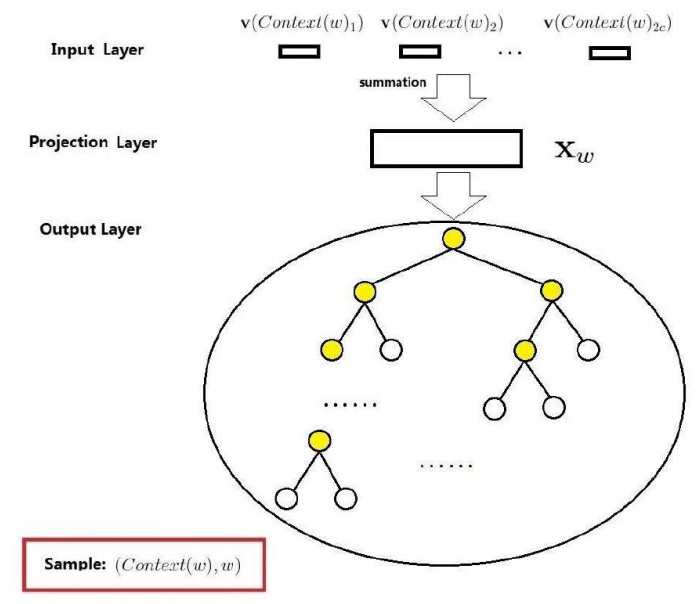
\includegraphics[width=1.0\textwidth]{cbow-hs}   
    \caption{\label{Fig:cbow-hs}CBOW with Hierarchical Softmax} 
\end{figure}

\par
在 Hierarchical Softmax 中,词汇表中的每个词对应二叉树中的一个叶子节点,从根节点到叶子节点的路径是确定的。
如果说把每一个非叶子节点看成是一个分类器,那么这个二叉树就相当于一个决策树,根据从根节点到叶子节点的路径,我们可以
计算在输入$X_w$的情况下的对应叶子节点对应词的条件概率,也就是我们上面希望建模的 Language Model 。
\par
对于一个训练样本,我们记当前词为w,那么我们需要说明如下的符号:
\begin{itemize}
\item[1.] $p^w$表示从根节点到w对应叶子节点的路径;
\item[2.] $l^w$表示路径$p^w$对应的节点个数;
\item[3.] $p_j^w(j \in [1, l^w])$表示路径$p^w$中的第j个节点;
\item[4.] $d_j^w(j \in [2, l^w])$表示路径中第j个节点对应的编码,对应值为0或者1,根节点不对应编码;
\item[5.] $\theta_j^w(j \in [1, l^w-1])$表示路径中第j个节点对应Logistic分类器参数,
          叶子节点并不产生分类,所以不对应$\theta$参数。
\end{itemize}
\par
在 Huffman Tree 的每个节点进行分类的时候,我们按照Logistic Classification的思路,每个非叶子节点
对应一个$\theta$参数,于是在该节点上输入被分类为正类的概率可表示为:
\[ \sigma(x_w^T \theta) = \frac{1}{1 + e^{-x_w^T \theta}} \]
那么该节点上被分为负类的概率则为:
\[ 1 - \sigma(x_w^T\theta)\]
word2vec中将编码为1的定义为负类,编码为0的定义为正类,其实这里的编码为0或者1,取决于在构造Huffman Tree
的时候,你怎么定义。在word2vec中,将两个兄弟节点中较小的编号为1。

\par
在训练样本中,给定一个(w, Context(w)),那么我们在投影层计算得到$x_w$之后,进入到输出层,也就是进入到
Huffman Tree 的结构中。这个时候,从根节点走到w对应叶子节点的过程中,共经历了$l^w-1$次分类,那么由
Context(w) 得到 w 的条件概率可以表示为:
\begin{equation}
\label{cbow-hs}
p(w|Context(w)) = \Pi_{j=2}^{l^w} p(d_j^w|x_w, \theta_{j-1}^w)
\end{equation}
那么对应的条件概率根据其在 Huffman Tree 上的编码确定
\begin{equation}
p(d_j^w|x_w, \theta_{j-1}^w)= \begin{cases}
\sigma(x_w^T \theta_{j-1}^w), \quad d_j^w=0
\\
1 - \sigma(x_w^T \theta_{j-1}^w), \quad d_j^w=1
\end{cases}
\end{equation}
按照 Logistic Regression 中的方式将上面的分段函数写在一起则可以表示为:
\[ p(d_j^w|x_w, \theta_{j-1}^w) = (\sigma(x_w^T \theta_{j-1}^w))^{1-d_j^w} \cdot (1-\sigma(x_w^T\theta_{j-1}^w))^{d_j^w} \]
\par
综合上式和(\ref{cbow-hs}),将其代入到(\ref{cobw-likelihood})中,我们可以得到log似然表示为:
\begin{align}
L &= \sum_{w \in C} log \Pi_{j=2}^{l^w}p(d_j^w|x_w, \theta_{j-1}^w)
\\
&= \sum_{w \in C} \sum_{j=2}^{l^w} \left( (1-d_j^w)log(\sigma(x_w^T \theta_{j-1}^w)) + d_j^w log(1-\sigma(x_w^T\theta_{j-1}^w)) \right)
\end{align}
\par
为了推导计算梯度方便,我们记上式大圆括号中的内容为
\begin{align}
L(w, j) = (1-d_j^w)log(\sigma(x_w^T \theta_{j-1}^w)) + d_j^w log(1-\sigma(x_w^T\theta_{j-1}^w))
\end{align}
\par
上式中,我们只有两个参数$(x_w, \theta_{j-1}^w)$,我们将$L(w, j)$对这两个参数进行求偏导,那么我们
可以得到下面的两个偏导公式:
\begin{align}
\frac{•}{•}
\end{align}


\subsection{Skip-gram Architecture}


\section{References}
\begin{itemize}
\item[1] Convolutional Neural Networks, \\
\url{http://andrew.gibiansky.com/blog/machine-learning/convolutional-neural-networks/} .
\item[2] 数据挖掘系列(10)卷积神经网络算法的一个实现, \\
\url{http://www.cnblogs.com/fengfenggirl/p/cnn\_ implement.html}.
\item[3] 受限波兹曼机(RBM)学习笔记, \\
\url{http://blog.csdn.net/itplus/article/details/19168937}
\end{itemize}

\end{document}
